%%%%%%%%%%%%%%%%%%%%%%%%%%%%%%%%%%%%%%%%%%%%%%%%%%%%%%%%%%%%%%%%%%
%%%%%%%%%%%%%%%%%%%%%%%%%%%%%%%%%%%%%%%%%%%%%%%%%%%%%%%%%%%%%%%%%%
%Packages
\documentclass[10pt, a4paper]{article}
\usepackage[top=3cm, bottom=4cm, left=3.5cm, right=3.5cm]{geometry}
\usepackage{amsmath,amsthm,amsfonts,amssymb,amscd, fancyhdr, color, comment, graphicx, environ}
\usepackage{float}
\usepackage{mathrsfs}
% \usepackage[math-style=ISO]{unicode-math}
% \setmathfont{TeX Gyre Termes Math}
\usepackage{lastpage}
\usepackage[dvipsnames]{xcolor}
\usepackage[framemethod=TikZ]{mdframed}
\usepackage{enumerate}
\usepackage[shortlabels]{enumitem}
\usepackage{fancyhdr}
\usepackage{indentfirst}
\usepackage{listings}
\usepackage{sectsty}
\usepackage{thmtools}
\usepackage{shadethm}
\usepackage{hyperref}
\usepackage{setspace}
\hypersetup{
    colorlinks=true,
    linkcolor=blue,
    filecolor=magenta,      
    urlcolor=blue,
}

%%%%%%%%%%%%%%%%%%%%%%%%%%%%%%%%%%%%%%%%%%%%%%%%%%%%%%%%%%%%%%%%%%
%                      Added Packages
%%%%%%%%%%%%%%%%%%%%%%%%%%%%%%%%%%%%%%%%%%%%%%%%%%%%%%%%%%%%%%%%%%

\usepackage{siunitx}
\usepackage{caption}
\usepackage[spanish]{babel}
\renewcommand{\spanishtablename}{Tabla}

%%%%%%%%%%%%%%%%%%%%%%%%%%%%%%%%%%%%%%%%%%%%%%%%%%%%%%%%%%%%%%%%%%
%%%%%%%%%%%%%%%%%%%%%%%%%%%%%%%%%%%%%%%%%%%%%%%%%%%%%%%%%%%%%%%%%%
%Environment setup
\mdfsetup{skipabove=\topskip,skipbelow=\topskip}
\newrobustcmd\ExampleText{%
An \textit{inhomogeneous linear} differential equation has the form
\begin{align}
L[v ] = f,
\end{align}
where $L$ is a linear differential operator, $v$ is the dependent
variable, and $f$ is a given non−zero function of the independent
variables alone.
}
\mdfdefinestyle{theoremstyle}{%
linecolor=black,linewidth=1pt,%
frametitlerule=true,%
frametitlebackgroundcolor=gray!20,
innertopmargin=\topskip,
}
\mdtheorem[style=theoremstyle]{Problem}{Problem}
\newenvironment{Solution}{\textbf{Solution.}}

\definecolor{codegreen}{rgb}{0,0.6,0}
\definecolor{codegray}{rgb}{0.5,0.5,0.5}
\definecolor{codepurple}{rgb}{0.58,0,0.82}
\definecolor{backcolour}{rgb}{0.95,0.95,0.92}

\lstdefinestyle{mystyle}{
    backgroundcolor=\color{backcolour},   
    commentstyle=\color{codegreen},
    keywordstyle=\color{magenta},
    numberstyle=\tiny\color{codegray},
    stringstyle=\color{codepurple},
    basicstyle=\ttfamily\footnotesize,
    breakatwhitespace=false,         
    breaklines=true,                 
    captionpos=b,                    
    keepspaces=true,                 
    numbers=left,                    
    numbersep=5pt,                  
    showspaces=false,                
    showstringspaces=false,
    showtabs=false,                  
    tabsize=2
}

\lstset{style=mystyle}
%%%%%%%%%%%%%%%%%%%%%%%%%%%%%%%%%%%%%%%%%%%%%%%%%%%%%%%%%%%%%%%%%%
%%%%%%%%%%%%%%%%%%%%%%%%%%%%%%%%%%%%%%%%%%%%%%%%%%%%%%%%%%%%%%%%%%
%Fill in the appropriate information below
\newcommand{\norm}[1]{\left\lVert#1\right\rVert}     
\newcommand\course{XXXX0000}                            % <-- course name   
\newcommand\hwnumber{0}                                 % <-- homework number
\newcommand\Information{Someone}                        % <-- personal information
%%%%%%%%%%%%%%%%%%%%%%%%%%%%%%%%%%%%%%%%%%%%%%%%%%%%%%%%%%%%%%%%%%
%%%%%%%%%%%%%%%%%%%%%%%%%%%%%%%%%%%%%%%%%%%%%%%%%%%%%%%%%%%%%%%%%%
%Page setup
\pagestyle{fancy}
\headheight 35pt
\lhead{\today}
\rhead{
\includegraphics[width=3cm]{images/logosimbolo-horizontal.png}}
\lfoot{}
\pagenumbering{arabic}
\cfoot{\small\thepage}
\rfoot{}
\headsep 1.2em
\renewcommand{\baselinestretch}{1.25}
%%%%%%%%%%%%%%%%%%%%%%%%%%%%%%%%%%%%%%%%%%%%%%%%%%%%%%%%%%%%%%%%%%
%%%%%%%%%%%%%%%%%%%%%%%%%%%%%%%%%%%%%%%%%%%%%%%%%%%%%%%%%%%%%%%%%%
%Add new commands here
\renewcommand{\labelenumi}{\alph{enumi})}
\newcommand{\Z}{\mathbb Z}
\newcommand{\R}{\mathbb R}
\newcommand{\Q}{\mathbb Q}
\newcommand{\NN}{\mathbb N}
\newcommand{\PP}{\mathbb P}
\DeclareMathOperator{\Mod}{Mod} 
\renewcommand\lstlistingname{Algorithm}
\renewcommand\lstlistlistingname{Algorithms}
\def\lstlistingautorefname{Alg.}
\newtheorem*{theorem}{Theorem}
\newtheorem*{lemma}{Lemma}
\newtheorem{case}{Case}
\newcommand{\assign}{:=}
\newcommand{\infixiff}{\text{ iff }}
\newcommand{\nobracket}{}
\newcommand{\backassign}{=:}
\newcommand{\tmmathbf}[1]{\ensuremath{\boldsymbol{#1}}}
\newcommand{\tmop}[1]{\ensuremath{\operatorname{#1}}}
\newcommand{\tmtextbf}[1]{\text{{\bfseries{#1}}}}
\newcommand{\tmtextit}[1]{\text{{\itshape{#1}}}}

\newenvironment{itemizedot}{\begin{itemize} \renewcommand{\labelitemi}{$\bullet$}\renewcommand{\labelitemii}{$\bullet$}\renewcommand{\labelitemiii}{$\bullet$}\renewcommand{\labelitemiv}{$\bullet$}}{\end{itemize}}
\catcode`\<=\active \def<{
\fontencoding{T1}\selectfont\symbol{60}\fontencoding{\encodingdefault}}
\catcode`\>=\active \def>{
\fontencoding{T1}\selectfont\symbol{62}\fontencoding{\encodingdefault}}
\catcode`\<=\active \def<{
\fontencoding{T1}\selectfont\symbol{60}\fontencoding{\encodingdefault}}

%%%%%%%%%%%%%%%%%%%%%%%%%%%%%%%%%%%%%%%%%%%%%%%%%%%%%%%%%%%%%%%%%%
%%%%%%%%%%%%%%%%%%%%%%%%%%%%%%%%%%%%%%%%%%%%%%%%%%%%%%%%%%%%%%%%%%
%Begin now!



\begin{document}

\begin{titlepage}
    \begin{center}
            
        \huge
        \textbf{Entrega 1: Evaluación de la Enfermedad de Parkinson Mediante Datos de Escritura a Mano}\\
        
        \huge
        Fundamentos de Deep Learning
        
        \vspace{1cm}
        Jeferson Gallo\\
        \large
        jeferson.gallo@udea.edu.co

        \vspace{1cm}
        
        \Large
       Estudiante de Maestía en Ingeniería de Telecomunicaciones\\
        Facultad de Ingeniería, Universidad de Antioquia

        \vspace{1.5cm}
        
        \begin{figure}[h!]
            \centering
            \includegraphics[width=8cm]{images/logosimbolo-vertical.png}
            %\caption{}
            %\label{fig:enter-label}
        \end{figure}
        
        \vfill
        \Large
        \today
            
    \end{center}
\end{titlepage}

%%%%%%%%%%%%%%%%%%%%%%%%%%%%%%%%%%%%%%%%%%%%%%%%%%%%%%%%%%%%%%%%%%
%%%%%%%%%%%%%%%%%%%%%%%%%%%%%%%%%%%%%%%%%%%%%%%%%%%%%%%%%%%%%%%%%%
%Start the assignment now
%%%%%%%%%%%%%%%%%%%%%%%%%%%%%%%%%%%%%%%%%%%%%%%%%%%%%%%%%%%%%%%%%%
%New problem
\newpage

\subsection*{Contexto}

La enfermedad de Parkinson (EP) es una enfermedad neurodegenerativa que afecta 
el sistema nervioso central mediante la pérdida progresiva de neuronas 
dopaminérgicas~\cite{ref1}. La dopamina es un neurotransmisor encargado del 
funcionamiento de las vías neuronales asociadas con la motivación, el estado de 
ánimo y el control motor~\cite{ref2}. Por esta razón, la EP puede causar síntomas 
motores como la bradicinesia (lentitud en los movimientos voluntarios), la rigidez 
muscular y los temblores en reposo. Estos síntomas afectan significativamente 
diferentes actividades de los pacientes como lo es la escritura a mano, ya que los 
procesos de escritura necesitan una alta coordinación de los músculos y tendones 
que conectan el antebrazo la muñeca y los dedos. Adicionalmente, las principales 
anomalías que se evidencia en la escritura son la micrografía (reducción anormal en 
el tamaño de la escritura) y la disgrafía (déficits en la producción grafomotora 
debido a una combinación de varios signos cardinales de la enfermedad de Parkinson)~\cite{ref32}.


\subsection*{Objetivo de Machine Learning}

En este proyecto se abordará una clasificación bi-clase entre pacientes con la enfermedad de Parkinson 
versus personas sanas mediante señales de escritura a mano, utilizando diferentes tareas como dibujos, 
escritos y una tarea compleja. Las imagenes correcpondientes a cada tarea se procesan mediante una red 
convolucional VGG16, la cual fue entrenada con la base de datos ImageNet, y a la cuál se le agregan dos 
capas densas completamente conectadas para realizar la clasificación entre parkinson y controles.
El objetivo principal se basa en determinar cual de las diferentes tareas de escritura me permite un mejor
modelamiento de la enfermedad de parkinson. 



\subsection*{Datos}

Los datos fueron recopilados utilizando una tableta Wacom Cintiq 13 HD con retroalimentación visual 
para los participantes y con una frecuencia de muestreo de 180 Hz. Esta tableta proporciona seis 
señales diferentes provenientes del proceso de escritura: la posición $x$, la posición $y$, la distancia 
desde la superficie hasta el lápiz (la posición $z$), la presión del lápiz, el ángulo azimut y la 
inclinación del lápiz (la altitud). Para la creación de las imagenes se utilian las señales $(x,y)$
las cuales corresponden a los trazos realizados sobre la superficie de la tablet. Un ejemplo de las
imágenes resultantes para algunas tareas se encuentran en la Figura~\ref{fig:db_images}.

Para este trabajo se tienen un total de 7 tareas dentro de las cuales se encuentran algunos escritos 
como el alfabeto, frase libre y nombre; tareas de dibuno como una linea curva, spiral y una casa; y 
finalmente se tiene una tarea compleja llamada rey. 


\begin{figure}
    \centering
    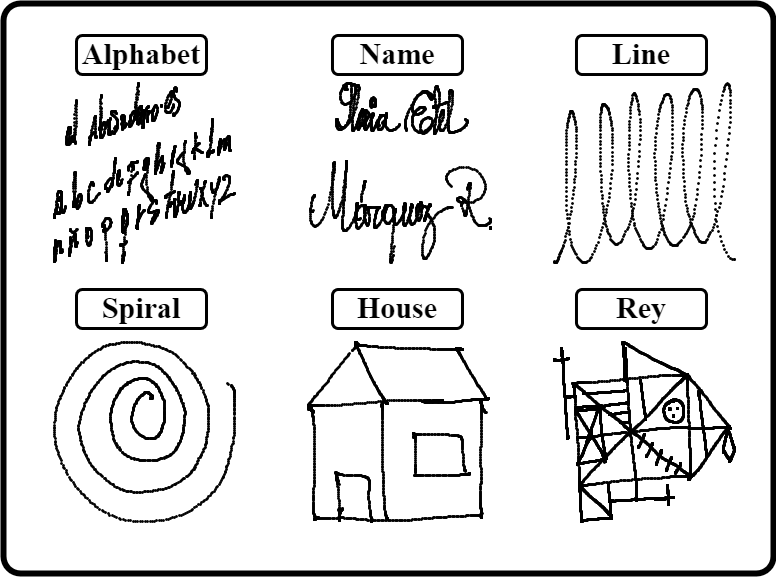
\includegraphics[width=0.6\textwidth]{images/HW_Tasks.png}
    \caption{Imágenes de la base de datos.}
    \label{fig:db_images}
\end{figure}


\subsection*{Metricas de desempeño}

En este proyecto se utilizarán métricas como la matriz de confusión, como también algunas 
métricas que se desprenden de esta. 

\subsubsection*{Matriz de confusión}

Es una matriz cuadrada donde el número de filas y columnas depende de la cantidad de clases 
diferentes que tenga el problema. Esta matriz organiza las predicciones correctas e incorrectas 
evidenciando el rendimiento del sistema para la predicción de cada clase. En problemas de 
clasificación bi-clase, la matriz de confusión es $2 \times 2$ donde en cada celda se pueden 
definir los siguientes términos:

\begin{itemize}
    \item \textit{Verdaderos positivos (TP, true positive):} es la cantidad de datos de la clase positiva que el sistema clasifico correctamente.

    \item \textit{Falsos positivos (FP, false positive):} son la cantidad de datos de la clase positiva que el sistema clasifico erróneamente como pertenecientes a la clase negativa.

    \item \textit{Verdaderos negativos (TN, true negative):} es el número de datos de la clase negativa clasificados correctamente por el sistema.

    \item \textit{Falsos negativos (FN, false negative):} es el número de datos de la clase negativa que el sistema clasifico erróneamente como pertenecientes a la clase positiva.
    
\end{itemize}

Además, otras métricas pueden ser estimadas de acuerdo con la información de la matriz de confusión:

\begin{itemize}
    \item \textit{Exactitud (acc, accuracy):} se define como la cantidad de aciertos en ambas clases sobre el total de datos.

    \begin{equation}
        acc = \frac{TP + TN}{TP + FP + TN + FN}
    \end{equation}

    \item \textit{Sensibilidad (S, sensitivity):} es la capacidad del sistema para clasificar la clase positiva.
    
    \begin{equation}
        S = \frac{TP}{TP+FN}
    \end{equation}

    \item \textit{Especificidad (E, especificity):} es la capacidad del sistema para clasificar la clase negativa.
    
    \begin{equation}
        E = \frac{TN}{TN+FP}
    \end{equation}

    \item \textit{Precisión (P, precision):} mide la proporción de muestras positivas predichas correctamente entre todas las muestras que se predicen como positivas.

    \begin{equation}
        P = \frac{TP}{TP+FP}
    \end{equation}

    \item \textit{F1-socre:} es la media armónica entre la precisión y la sensibilidad, la cual permite obtener una medición balanceada del desempeño del modelo.

    \begin{equation}
        F1-score = 2 \times \frac{P \times S}{P+S}
    \end{equation}
    
\end{itemize}


\bibliographystyle{splncs04}
\bibliography{refs}

\end{document}

%%%%%%%%%%%%%%%%%%%%%%%%%%%%%%%%%%%%%%%%%%%%%%%%%%%%%%%%%%%%%%%%%%
%%%%%%%%%%%%%%%%%%%%%%%%%%%%%%%%%%%%%%%%%%%%%%%%%%%%%%%%%%%%%%%%%%
